\chapter{ Allgemeines}
%\addcontentsline{toc}{section}{Allgemeines}
%\setcounter{section}{1}
%\setcounter{equation}{0}
\section{Einführung}
Das vorliegende Flughandbuch wurde erstellt, um Piloten und Ausbildern alle notwendigen Informationen für einen sicheren, zweckmäßigen und leistungsoptimierten Betrieb des Motorseglers B13 zu geben.\\
\newline
Das Handbuch enthält zunächst alle Daten die dem Piloten aufgrund der Bauvorschrift JAR-22 zur Verfügung stehen müssen. Es enthält darüber hinaus jedoch eine Reihe weiterer Daten und Betriebshinweise, die aus Herstellersicht für den Piloten von Nutzen sein können.

\section{Zulassungsbasis}
Der Motorsegler B13 wird im Rahmen einer "`Vorläufigen Verkehrszulassung"' betrieben. Die Zulassungsbasis stellt die JAR-22 vom 15. März 1982.\\
\newline
Lufttüchtigkeitsgruppe: Utility
\newpage
\section{Warnungen, wichtige Hinweise und Anmerkungen}
Die nachfolgenden Definitionen gelten für Warnungen, wichtige Hinweise und
Anmerkungen im Flughandbuch.\\
\newline
\newline
\begin{color}{red}
\large{\underline{Warnung}}\\
bedeutet, dass die Nichteinhaltung einer entsprechend gekennzeichneten Verfahrensvorschrift zu einer unmittelbaren oder erheblichen Beeinträchtigung der Flugsicherheit führt.
\end{color}\\
\newline
\begin{color}{forestgreen}
\large{\underline{Wichtiger Hinweis}}\\
bedeutet, dass die Nichteinhaltung einer entsprechend gekennzeichneten Verfahrensvorschrift zu einer geringfügigen oder einer mehr oder weniger langfristig eintretenden Beeinträchtigung der Flugsicherheit führt.
\end{color}\\
\newline
\begin{color}{blue}
\large{\underline{Anmerkung}}\\
soll die Aufmerksamkeit auf Sachverhalte lenken, die nicht unmittelbar mit der Sicherheit zusammenhängen, die aber wichtig oder ungewöhnlich sind.
\end{color}

\section{Beschreibung und technische Daten}
Die B13 ist ein doppelsitziger Motorsegler mit einem gedämpften T-Leitwerk, 4-teiligen Tragflächen, nebeneinander angeordneten Sitzen, dreistöckigen Oberseiten-Bremsklappen und einem gefederten Hauptfahrwerk.\\
\newline
Die B13 wurde für wissenschaftliche Zwecke und für den Leistungsflug entworfen.
\newpage
\textbf{Technische Daten}\\

\begin{longtable}{l l l}
Besatzung & & 1+1\\
 & & \\
 Tragflügel & & \\
  & Spannweite & $\unit[23,20]{m}$\\
  & Fläche & $\unit[18,95]{m^2}$\\
  & Streckung & $28,4$ \\
  & Ersatzflügeltiefe & $\unit[873]{mm}$ \\
  & Einstellwinkel & $\unit[0]{^{\circ}}$ \\
  & Pfeilung zur $\unit[25]{\%}$-Linie & $\unit[-0,3]{^{\circ}}$ \\
  & V-Stellung & $\unit[1]{^{\circ}}$\\
  & Verwindung & $\unit[0]{^{\circ}}$\\
  & Profil & HQ 41/14,35\\
  & Klappentiefe & $\unit[17,5]{\%}$ \\
  & & \\
 Rumpf & & \\
 & Länge & $\unit[8,55]{m}$\\
 & Breite & $\unit[1,28]{m}$\\
 & Höhe & $\unit[0,90]{m}$ \\
 & & \\
 Höhenleitwerk & & \\
 & Spannweite & $\unit[3,10]{m}$\\
 & Fläche & $\unit[1,457]{m^2}$\\
 & Profil & FX 71-L-150/25 \\
 & & \\
 Seitenleitwerk & & \\
 & Höhe & $\unit[1,70]{m}$ \\
 & Fläche & $\unit[1,71]{m^2}$\\
 & Profil & FX 71-L-150/30\\
 & & \\
 Bremsklappen & & \\
 & Spannweite & $\unit[1,50]{m}$\\
 & Höhe & $\unit[250]{mm}$ \\
 & Fläche & $\unit[0,75]{m^2}$\\
 & & \\
 Fahrwerk & & \\
 & Hauptrad, einziehbar & $380$ x $150$\\ 
 & & $\unit[3-3,5]{bar}$\\
 & Heckrad, fest & $210$ x $65$ \\ 
 & & $\unit[2,5-2,8]{bar}$\\
 & Radstand & $\unit[5,60]{m}$\\
 & & \\
 Massen & & \\
 & Leermasse & s. Wägebericht\\
 & Höchstmasse & $\unit[820]{kg}$\\
 & Flächenbelastung min/max & $\unit[34,7]{\frac{kg}{m^2}}$/$\unit[43,3]{\frac{kg}{m^2}}$\\
 & & \\
 Flugleistungen & & \\
 & bei Flugmasse $\unit[765]{kg}$ & \\
 & beste Gleitzahl (WK +1) & $45,4$ $(\unit[95]{\frac{km}{h}})$ \\
 & geringstes Sinken (WK +1) & $\unit[0,56]{\frac{m}{s}}$ $ (\unit[90]{\frac{km}{h}})$

\end{longtable}
\newpage
Die B13 ist mit einem hochwertigen und leistungsstarken elektrischem Antriebssystem ausgestattet. Das Antriebssystem basiert in weiten Teilen auf dem FES System, mit Änderungen am Antriebsmotor, Inverter, Propeller und Propellerschlitten sowie der Batteriekapazität.\\

Hauptbestandteile des Antriebssystems sind:
\begin{itemize}
\item Brushless Elektromotor EMRAX 208 LV AC
\item Motorsteuerungseinheit Emsiso emDrive500
\item Nach vorn faltbarer Propeller mit Ausfahreinheit und Steuerung
\item FES GEN 2 75Ah Akkupacks, mit integriertem BMS (Batteriemanagementsystem)
\item Ladegerat 1200W
\item FCU (FES Steuerungseinheit) Instrument
\item LXUI Box mit Shunt (als Messgerät für Strom und Spannung)
\item FCC Box (FES Schaltkreis)
\item Leistungsschalter
\item DC/DC Wandler (wandelt Hochspannung in 12V)
\end{itemize}



\section{Dreiseitenansicht}
\vspace{4cm}
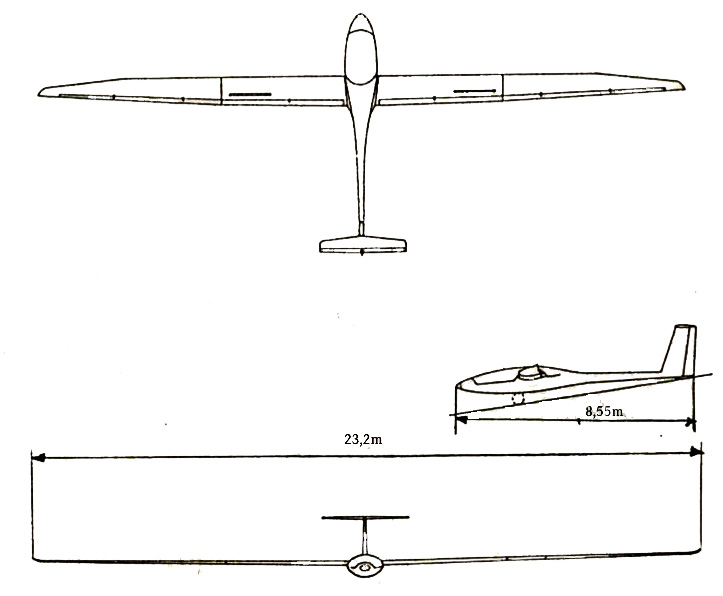
\includegraphics[width=\textwidth]{3seiten.jpg}

\section{Abkürzungen}
\begin{tabular}{p{0.2\textwidth}p{0.7\textwidth}ll} 
CAS & kalibrierte Eigengeschwindigkeit (calibrated airspeed): IAS eines Segelflugzeugs, die um Messfehler korrigiert ist; die kalibrierte Eigengeschwindigkeit entspricht der wahren Eigengeschwindigkeit (TAS) auf Meereshöhe unter den Bedingungen der Standardatmosphare \\
C.G. & Schwerpunkt (center of gravity)\\
daN & Decanewton \\
h & Stunde \\
IAS & angezeigte Eigengeschwindigkeit (indicated airspeed): relative Geschwindigkeit eines Segelflugzeugs zur umgebenden Luftmasse, die auf dem Fahrtmesser angezeigt wird \\
m & Meter \\
kg & Kilogram  \\
km & Kilometer \\
s & Sekunde \\
Ltr & Liter \\
\end{tabular}

\section{Einheitenumrechnung}
\begin{tabular}{p{0.35\textwidth}p{0.65\textwidth}ll}
1 bar & = 14,5 pounds per square inch (psi);\\
1 decanewton (daN)& = 2,25 pounds force;\\
1 Kilogram (kg) & = 2,2 pounds (lbs);\\
1 meter (m) & = 39,4 inches (in.) = 3,28 feet (ft.);\\
1 Millimeter (mm) & = 0,0394 inches (in.);\\
1 Liter & = 0,2642 U.S. gal; \\ 
1 Quadratmeter (m$^2$) &= 10,764 sq.ft;\\
1 kg/m$^2$ &= 0,204 lbs/sq.ft;\\
1 m/s & = 1,944 Knoten (kts);\\
1 km/h & = 0,5396 kts;\\
1 kW & = 1,34 HP.
\end{tabular}
